\documentclass{article} % For LaTeX2e
\usepackage{nips11submit_e,times,amsmath,amsfonts, graphicx, subfigure,amssymb}
%\documentstyle[nips10submit_09,times,art10]{article} % For LaTeX 2.09


\title{Unlabeled graph classification}


\author{
Joshua T.~Vogelstein\thanks{ Use footnote for providing further information
about author (webpage, alternative address)---\emph{not} for acknowledging
funding agencies.} \\
Department of Applied Mathematics and Statistics\\
Johns Hopkins University\\
Baltimore, MD 21218 \\
\texttt{joshuav@jhu.edu} \\
\And
John M.~Conroy \\
Affiliation \\
Address \\
\texttt{conroyjohnm@gmail.com} \\
\AND
Glen A.~Coppersmith \\
Affiliation \\
Address \\
\texttt{coppersmith@jhu.edu} \\
\And
Mark Dredze \\
Affiliation \\
Address \\
\texttt{mdredze@cs.jhu.edu} \\
\And
R.~Jacob Vogelstein \\
Affiliation \\
Address \\
\texttt{Jacob.Vogelstein@jhuapl.edu} \\
\And
Carey E.~Priebe \\
Affiliation \\
Address \\
\texttt{cep@jhu.edu} \\
}


\newcommand{\fix}{\marginpar{FIX}}
\newcommand{\new}{\marginpar{NEW}}

\newcommand{\jv}{Joshua Vogelstein}
\newcommand{\jhu}{Johns Hopkins University}
%\newcommand{\hp}{https://jshare.johnshopkins.edu/jvogels3/public_html/}
\newcommand{\ema}{joshuav@jhu.edu}

\newcommand{\eqdef}{\overset{\triangle}{=}}
\newcommand{\D}[2]{\frac{\partial #1}{\partial #2}}
\newcommand{\DD}[2]{\frac{\partial ^2 #1}{\partial #2 ^2}}
\newcommand{\DDD}[3]{\frac{\partial ^2 #1}{\partial #2 \partial #3}}
\newcommand{\Di}[2]{\frac{\partial ^i #1}{\partial #2 ^i}}
\newcommand{\grad}{\nabla}
\newcommand{\Hess}{\nabla\nabla}

\providecommand{\ve}[1]{\boldsymbol{#1}}
\providecommand{\norm}[1]{\left \lVert#1 \right  \rVert}
\providecommand{\deter}[1]{\lvert #1 \rvert}
\providecommand{\abs}[1]{\left \lvert #1 \right \rvert}
\newcommand{\argmax}{\operatornamewithlimits{argmax}}
\newcommand{\argmin}{\operatornamewithlimits{argmin}}
\newcommand{\T}{^{\ensuremath{\mathsf{T}}}}           % transpose
\newcommand{\EE}{\mathbb{E}}           % expected value
\newcommand{\PP}{\mathbb{P}}           % probability
\newcommand{\II}{\mathbb{I}}           % indicator function
\newcommand{\QQ}{\mathbb{Q}}           
\newcommand{\SSS}{\mathbb{S}}           

\newcommand{\bth}{\ve{\theta}}
\newcommand{\bTh}{\ve{\Theta}}
\newcommand{\hbth}{\widehat{\thet}}

\providecommand{\mc}[1]{\mathcal{#1}}
\providecommand{\mb}[1]{\boldsymbol{#1}}
\providecommand{\mbb}[1]{\mathbb{#1}}
\providecommand{\mv}[1]{\vec{#1}}
\providecommand{\mh}[1]{\hat{#1}}
\providecommand{\mt}[1]{\widetilde{#1}}
\providecommand{\mhc}[1]{\hat{\mathcal{#1}}}
\providecommand{\mhb}[1]{\hat{\boldsymbol{#1}}}
\providecommand{\mvb}[1]{\vec{\boldsymbol{#1}}}
\providecommand{\mtb}[1]{\widetilde{\boldsymbol{#1}}}

\newcommand{\Real}{\mathbb{R}}
\newcommand{\conv}{\rightarrow}

\newcommand{\mcE}{\mathcal{E}}
\newcommand{\mcT}{\mathcal{T}}
\newcommand{\mcG}{\mathcal{G}}
\newcommand{\mcM}{\mathcal{M}}
\newcommand{\mcL}{\mathcal{L}}
\newcommand{\hatmcE}{\widehat{\mcE}}
\newcommand{\hatp}{\widehat{p}}
\newcommand{\hatP}{\widehat{P}}
\newcommand{\hatQ}{\widehat{Q}}
\newcommand{\hatL}{\widehat{L}}
\newcommand{\mhP}{\widehat{\PP}}
\newcommand{\tildeA}{\widetilde{A}}
\newcommand{\GG}{\mathbb{G}}
\newcommand{\qap}{\texttt{QAP} }
\newcommand{\qapa}{\texttt{QAP$_1$} }
\newcommand{\qapn}{\texttt{QAP$_n$} }
\newcommand{\qapb}{\texttt{QAP$_{100}$} }


%\nipsfinalcopy % Uncomment for camera-ready version

\begin{document}

 
\maketitle

\begin{abstract}
Because graphs can encode more information in their structure than vectors, they are becoming increasingly popular data structures for representing information.  While the last century has witnessed the development of a plethora of statistical tools for the analysis of data, the vast majority of these tools natively operate in vector spaces, not graph spaces.  Thus, even relatively simple statistical inference tasks, such as two-way classification,  are essentially absent for graph data.  In this work, we propose a number of complementary algorithms to classify graphs, with special attention to the possibility of an unknown vertex labeling function.  Since exactly solving the graph-matching problem is currently computational intractable, we consider several approximate approaches.  We introduce a multiple-restart Frank-Wolfe approach to solving the graph matching problem by formulating it as a quadratic assignment problem.  Although this approach has superior performance than previous state-of-the-art approaches to the graph matching problem, even when it ``should'' do well in classification problems, it is outperformed by a graph invariant strategy.  This is just the beginning. 
\end{abstract}

\section{Introduction}


\qapa and \qapn and \qapb.
The statistical analysis of collections of graphs is becoming an increasingly popular desideratum [cite].  Specifically, we consider the following idealized and simplified scenario. Let $\GG: \Omega \mapsto \mc{G}$ be a graph-valued random variable taking values $G\in \mc{G}$. Each graph is a 4-tuple: $G=(\mc{V},\mc{E},\alpha_V,\alpha_E)$, where $\mc{V}$ is a set of $|\mc{V}|=V$ vertices, $\mc{E}$ is a set of $|\mc{E}|=E$ edges, $\alpha_V: \mc{V} \mapsto \mc{A}_V$ is a vertex labeling function, and $\alpha_E: \mc{E} \mapsto \mc{A}_E$ is an edge attributing function (for example, edge weights).  Given a graph, if $\mc{A}_E$ is univariate, one can construct an adjacency matrix representation, $A \in \mc{A}_E^{V \times V}$ (generalizations to adjacency tensors are straightforward).  Let $Y$ be a Bernoulli covariate: $Y: \Omega \mapsto \{0,1\}$, yielding graph two-way \emph{classification} problem.  Given a collection of graphs and associated covariates,  we assume they were jointly sampled independently and identically from some true but unknown distribution, $\{(\GG_i,Y_i)\}_{i \in [n]} \sim F_{\GG,Y}(\cdot; \theta)$.  Note that $F_{\GG,Y}(\cdot; \bth)$ is but one of a (possibly infinite) set of distributions, collectively comprising the model: $\mc{F_{\GG,Y}}=\{F_{\GG,Y}(\cdot; \bth) : \theta \in \bTh\}$, where $\bTh$ is the set of feasible parameters.  The goal of such an analysis is to learn about the relationship between $\GG$ and $Y$.   Standard classification techniques fail in this domain as they typically require classifying finite dimensional Euclidean objects ($G \in \Real^d$), whereas the object of interest here are graphs ($G \in \mc{G} \nsubseteq \Real^d$).   In this work, therefore, we propose novel extension of classification algorithms appropriate for the graph domain.



\section{Graph Classification} % (fold)
\label{sec:graph_classification}


The graph classification problem may be stated thusly: given $\mc{T}_n=\{(\GG_i,Y_i)\}_{i \in [n]} \sim F_{\GG,Y}(\cdot; \theta)$ and a new graph, $\GG$, estimate the new graph's corresponding class, $Y$.  Given an appropriately defined loss-function, such as misclassification rate: $L_h=\PP[h(\GG) \neq Y]$, one can then search for the algorithm $h^* \in \mc{H}$ that minimizes the loss function of interest:
\begin{align}
	h^* = \argmin_{h \in \mc{H}} \PP[h(\GG) \neq Y].
\end{align}
In general, $h^*$ is unavailable and dependent on the model, $\mc{F}_{\GG,Y}$.  Instead, one can therefore utilize training data, $\mc{T}_n$, to obtain $\mt{h}$, an approximation to $h^*$:
\begin{align}
	\mt{h} \approx \argmin_{h \in \mc{H}} \PP[h(\GG) \neq Y | \mc{T}_n],
\end{align}
where $\approx$ indicates that in general, we will not be able to find the actual minimum in the set $\mc{H}$. Regardless, any approach necessarily estimates a decision boundary in the space of graphs separating them into two classes.  We consider a few distinct such approaches to constructing such a decision boundary:

% \subsection{Graph dissimilarity based approach approach} % (fold)
% \label{sub:_k__n_nearest_neighbor_approach}

% \subsection{Graph dissimilarity based approach approach} % (fold)
% \label{sub:_k__n_nearest_neighbor_approach}

\begin{description}
	\item[Graph dissimilarity approach] Define a dissimilarity on graph spaces: $d: \mc{G} \times \mc{G} \mapsto \Real_+$, in which one can compute the dissimilarity between any pair of graphs [cite]. Given an adjacency matrix representation, many such dissimilarities are possible (e.g., graph edit distance, Hamming distance, etc.).  It is becoming increasingly popular to use a \emph{graph kernel}, $\kappa(G,G')=\langle \phi(G), \phi(G') \rangle$, as the dissimilarity [cite] ($\langle \cdot, \cdot \rangle$ indicates a dot-product).  Graph kernels have a number of desirable properties, perhaps most notably, that one can then use standard \emph{kernel machines} to classify.	Whether or not one uses a graph kernel, given such a dissimilarity, standard classification algorithms, including $k_n$ nearest neighbor ($k$NN) algorithms [cite] and interpoint-dissimilarity matrix based algorithms [cite], can be straightforwardly applied.  
	\item[Graph model approach] Factorize the joint distribution on graphs and classes into a (i) class-conditional random graph model: $\mc{F}_{\GG  | Y} = \{F_{\GG|Y}[\cdot; \bth_Y] : \bth_Y \in \bTh\}$, and (ii) a class prior, $F_Y[\cdot; \pi_Y] \in \mc{F}_Y$.  Given such a factorization, one could then, for instance, estimate $\{\bth,\pi\}$ and then use standard model-based classifiers (for example, the Bayes plugin classifier) [VogelsteinPriebe11]. 
	\item[Graph embedding approach] Define an embedding of graphs into finite dimensional Euclidean space: $\phi: \mc{G} \mapsto \Real^d$.  Once in $\Real^d$, one can apply one of many possible standard machine learning or other such approaches [Bunke]. 
\end{description}



% section graph_classification (end)
\section{Unlabeled sticky wicket}

In certain graph classification problems the vertex labeling function, $\alpha_V$, is unknown.  In such scenarios, one must (either implicitly or explicitly) deal with the \emph{graph matching} (GM) problem.  In words, graph matching is the operation of finding a set of labels for a collection of vertices on multiple graphs.  For the graph classification setting, we require an \emph{approximate} GM approach [Conte04], as we do not expect, in general, for graphs to be isomorphic to one another; rather, we expect graphs within the same class to be ``similar'' to one another.  We consider two complimentary approaches to approximate graph matching.
\begin{description}
	\item[Adjacency matrix space approach]  In this representation, GM can be considered a special case of a quadratic assignment problem (QAP) [cite].   Unfortunately, no polynomial time algorithm is known to solve QAP, although much work has been devoted to this problem [cite]. Fortunately, efficient and approximate QAP solvers, such as the Frank-Wolfe (FW) algorithm [cite], are readily available.  Given an approximate assignment of each graph, one can use any of the above classification approaches.
	\item[Graph invariant (GI) approach] A graph invariant is any function that maps a graph to a scalar whose value is independent of the vertex labeling, $T: (\mc{V},\mc{E}) \mapsto \Real$.  By defining a set of GIs, one can embed a collection of graphs into an invariant space.  This could be considered a special case of the ``Graph embedding approach'' to classification described above.		
\end{description}



\section{Methods} % (fold)
\label{sec:methods}

\subsection{QAP Approach} % (fold)
\label{sec:quadratic_assignment_problem}

In the adjacency matrix approach, we first use an approximate QAP approach to approximate the GM problem.  Then, given the estimated labels, we can implement a $k$NN classifier. 

The QAP is defined by the following, where we seek to find a permutation matrix, $\mh{Q}$, such that
 \begin{align} \label{eq:QAP}
	Q_{QAP}(A,B)=Q_{QAP} = \argmin_{Q \in \mc{Q}} \norm{Q A Q\T - B}^2_F
\end{align}
where $A$ and $B$ are adjacency matrix representations of two different graphs.  A bit of linear algebra [HornJohnson] shows that Eq \eqref{eq:QAP} can be simplified:
\begin{align} \label{eq:qap}
	Q_{QAP} &= \argmin_{Q \in \mc{Q}} \norm{Q A Q\T - B}^2_F = \argmin_{Q \in \mc{Q}} - tr(B\T QAQ\T) - tr(QAQ\T B),			
\end{align}
which is equivalent to the standard representation of the quadratic assignment problem \cite{}:
\begin{align}
	\mh{\sigma}= \argmin_{\sigma} a_{\sigma(i), \sigma(j)} b_{ij} = \argmin_{q \in \mc{Q}} q_{ij} a_{ij}, q_{ji} b_{ij}
\end{align}
where $\sigma$ is a permutation, that is, $\sigma: [n] \mapsto [n]$.  As hinted at above, solving Eq. \eqref{eq:qap} is NP-Incomplete (not known to belong either to P or NP).  Because the primary difficulty is the discrete, non-convex constraint set, it is natural to consider an approximate solution with the constraints relaxed.  And because the set of permutation matrices is a subset of the doubly stochastic matrices, we define the approximate quadratic assignment problem:
\begin{align} \label{eq:tqap}
	Q_{AQAP} = \argmin_{Q \in \mc{D}} \norm{Q A Q\T - B}^2_F,
\end{align}
where $\mc{D}$ is the set of doubly stochastic matrices.  Note that when the permutation matrix constraint it relaxed, the equivalence relation shown in Eq. \eqref{eq:qap} no longer holds, that is:
\begin{align} \label{eq:nqap}
	\argmin_{Q \in \mc{D}} \norm{Q A Q\T - B}^2_F \neq \argmin_{Q \in \mc{D}} - tr(B\T QAQ\T) - tr(QAQ\T B).
\end{align}
Nonetheless, we proceed by trying to solve Eq. \eqref{eq:tqap}, considering it an auxiliary function for which we can compute gradients and ascend a likelihood, unlike the permutation constrained case.  

The Frank-Wolfe (FW) algorithm is a successive linear programming (SLP) \cite{} algorithm for nonlinear programming problems, specifically, for quadratic problems with linear (equality and/or inequality) constraints. Let $f(Q)=\norm{QAQ\T-B}_F^2$.  With each step $k$, the gradient of $f$ with respect to $Q$ is given by:
\begin{align} \label{eq:grad}
	\nabla_Q^{(k)} = \partial f / \partial Q^{(k)} =  A Q^{(k)} B\T + A\T Q^{(k)} B, 
\end{align}
see \cite{MDS} pg. 168 for details. Instead of directly ascending this gradient, we traverse the direction of the doubly stochastic matrix closest to this gradient. Noting that that direction may be computed by the dot-product operator, we have:
\begin{align}\label{eq:LAP}
	W^{(k)} = \argmin_{W^{(k)} \in \mc{D}} \langle \nabla_Q^{(k)},W^{(k)} \rangle. %  \sum_{i,j=1}^m 	\left( 	\nabla_Q^{(k)}\circ W^{(k)} \right)_{ij}.
\end{align}
Although $W^{(k)}$ is constrained only to be a doubly stochastic matrix, it is guaranteed to be a permutation, because the permutation matrices are the vertices of the set of doubly stochastic matrices (and minima are necessarily at the vertices).  Note that Eq. \eqref{eq:LAP} is a linear assignment problem (LAP) \cite{}.  The Hungarian algorithm is an efficient algorithm for finding the global optimum of any LAP in $\mc{O}(V^3)$ \cite{}.\footnote{More efficient algorithms are available for certain special cases, that is, whenever the matrix-vector multiplication operation is fast (for example, when both $A$ and $B$ are sparse).} Given this direction, one can then perform a line search to find the doubly stochastic matrix that minimizes the objective function along that direction:
\begin{align}
	\alpha^{(k)} = \argmin_{\alpha \in [0,1]} f(Q^{(k)} + \alpha^{(k)} W^{(k)})
\end{align}
This can be performed exactly, because $f$ is a quadratic function.  Finally, the new estimated doubly stochastic matrix is given by:
\begin{align}\label{eq:update}
	Q^{(k+1)} = Q^{(k)} + \alpha^{(k)} W^{(k)}
\end{align}
Eqs. \eqref{eq:grad}--\eqref{eq:update} are iterated until convergence, computational budget limits, or some other stopping criterion is met.  Note that while $Q^{(k+1)}$ is not a permutation matrix, we do not project $Q^{(k+1)}$ back onto the set of permutation matrices between each iteration, as that projection is a LAP, and requires $\mc{O}(n^3)$ time. At convergence, however, we have $\mh{Q}_{AQAP}$, which we project onto the set of permutation matrices:
\begin{align}
	\mh{Q}_{QAP} = \argmin_{Q \in \mc{Q}} \langle \mh{Q}_{AQAP}, Q \rangle,
\end{align}
which is our approximate solution to QAP.  Note that FW will not generally achieve the global optimal even of Eq. \eqref{eq:tqap}, because $f$ is not necessarily positive definite.  This is clear upon computing the Hessian of $f$  with respect to $Q$:
\begin{align}
	\nabla_Q^2  =  B \otimes A + B\T \otimes A\T,
\end{align}
where $\otimes$ indicates the Kronecker product. This means that the initialization, $Q^{(0)}$, will be important.  While any doubly stochastic matrix would be a feasible initial point, two choices seem natural: (i) the ``flat doubly  stochastic matrix,'' $J=\ve{1}\T \ve{1}/V$, which is the middle of the feasible region, and (ii) the identity matrix, which is actually a permutation matrix.  Therefore, if we run the FW algorithm once, we always start with one of those two.  If we use multiple restarts, each initial point is ``near'' the flat matrix.  Specifically, we sample $J'$, a random doubly stochastic matrix using 10 iterations of Sinkhorn rebalancing, and let $Q^{(0)}=(J+J')/2$.  We refer to multiple re-starts of \qap with subscripts, that is, the performance of \qapn is the best QAP of $n$ pseudo-random re-starts.  



\subsubsection{\texttt{$k$NN} $\circ$ \qap} % (fold)
\label{ssub:_k_nn_circ_qap}


We use the following algorithm to utilize the above approach within a $k$NN classification framework.  Given a test adjacency matrix, $A$, find $\mh{Q}_i^A=\mh{Q}_{QAP}(A,B_i)$ for all $n$ training adjacency matrices, $\{B_i\}_{i \in [n]}$.  Given these solutions, let $\mt{A}_i=\mh{Q}_i^A A {\mh{Q}_i^A}{}\T$ for all $i$. Given a suitable dissimilarity $d: \mc{A}_E^{V\times V} \times \mc{A}_E^{V\times V} \mapsto \Real_+$, one can compute $d(\mt{A}_i,B_i)$ for all $i \in [n]$, and sort them: $d_{(1)} \leq d_{(2)} \leq \cdot \leq d_{(n)}$.  Let the $k_n$ nearest neighbors of $A$ be the graphs with the $k_n$ smallest distances, $\{d_{(1)},\ldots, d_{(k)}\}$.\footnote{Note that $k_n$ is a function of $n$, typically chosen so that as $n \conv \infty$, $k \conv \infty$ but $k/n \conv 0$, to satisfy the universal consistency proofs [cite].}  The estimated class of the training sample $A$ is then the plurality class of the $k_n$ nearest neighbors: $\mh{y}=\argmax_{y} \II\{\sum_{i \in [k_n]} y_{(i)} = y \}$.

% subsubsection _k_nn_circ_qap (end)


\subsubsection{\texttt{BPI}$\circ$\qap} % (fold)
\label{ssub:bayes_plugin_circ_qap}


To utilize a Bayes plugin (BPI) classifier with \qap, we take the following strategy.  First, we assume an independent edge random graph model for each class: $F_y=\prod_{(u,v) \in \mc{E}}p_{uv|y}^{a_{uv}} (1-p_{uv|y})^{(1-a_{uv|y})}$, where $\{p_{uv|y}\}$ are the likelihood parameters.  For simplicity, we assume class prior probabilities are equal, $\PP[Y=1]=\PP[Y=0]=1/2$.  Given a test adjacency matrix, $A$,  do QAP$_1$ with respect to a single training graph from each class: $\mh{Q}_i^A=\mh{Q}_{QAP}(A,B_i)$ for $i=0,1$.  Then, compute the likelihood of $A$ coming from each class, using the true parameters.  Because class-prior probabilities are $1/2$, the likelihood is equal to the posterior, so $\mh{y}=\argmax_y \PP[Y=y | A; \{p_{uv|y}\}]$. This procedure fundamentally only uses \emph{two} training samples, one from each class. 

% subsubsection bayes_plugin_circ_qap (end)

% subsection graph_isomorphism_approach (end)

\subsection{Graph invariant approach} % (fold)
\label{sub:graph_invariant_approach}

In the graph invariant approach, we first define a set of $d$ graph invariants: (i) , (ii) , (iii)....  For each graph $G_i$ in the training set, we compute a graph invariant vector: $\mb{T}_i: \mc{G} \mapsto \Real^d$.  We stack these $n$ $d$-dimensional vectors to form a matrix $\mb{T} \in \Real^{n \times d}$. We then whiten this matrix to control for the divergence means and scales of the various graph invariants, $\mtb{T}=(\mb{T}-\mb{\mu}) \mb{\Sigma}^{-1}$, where $\mb{\mu}$ and $\mb{\Sigma}$ are the mean and variance of $\mb{T}$, respectively.  Now, to estimate the class of a test graph, we first compute its invariant vector, $\mb{t}$, and normalize it appropriately.  Then, we can apply a standard $k$NN algorithm, given a suitably defined dissimilarity (and rule for $k_n$).


% subsection graph_invariant_approach (end)

% section methods (end)


\section{Results}

\subsection{QAP benchmarks vs. PATH algorithm}

Before comparing the \qap and GI approach, we first compare the performance of \qapn with recent state-of-the-art approaches on the QAP benchmark library [Cela07 \# 38 in PATH paper].  Specifically, [PATH] reported improved performance in all but two cases, in which the QPB method of Cremers et al. [18 in PATH] achieved a lower minimum.  We compare \qapn with the previous best performing algorithm.  In \emph{all} cases, \qapb outperforms the previous best result.  In 12 out of 16 cases $75\%$, the simple \qapa algorithm outperforms the others (starting with the flat doubly stochastic matrix).  See Table \ref{tab:fwpath} and Figure \ref{fig:fwpath} for quantitative results.


\begin{table}[h!]
\caption{Comparison of Frank-Wolfe with Minimum Solution and Previous State-of-the-Art (PSOA)}
\begin{center}
\begin{tabular}{|r|r|r||r|r|r|r|r|}
\hline
\# & Problem  &   Min    & \qapb & \texttt{QAP}$_{3}$ & \texttt{QAP}$_{2}$ & \qapa & PSOA\\
\hline
1&    chr12c &   11156 &   12176 &   13072 &   13072 &   13072 &   18048\\
2&    chr15a &    9896 &    9896 &   17272 &   17272 &   27584 &   19086\\
3&    chr15c &    9504 &   10960 &   14274 &   14274 &   17324 &   16206\\
4&   chr20b &    2298 &    2786 &    3068 &    3068 &    3068 &    5560\\
5&    chr22b &    6194 &    7218 &    7876 &    7876 &    8482 &    8500\\
6&    esc16b &     292 &     292 &     294 &     294 &     320 &     296\\
7&     rou12 &  235528 &  235528 &  238134 &  253684 &  253684 &  256320\\
8&     rou15 &  354210 &  356654 &  371458 &  371458 &  371458 &  381016\\
9&     rou20 &  725522 &  730614 &  743884 &  743884 &  743884 &  778284\\
10&    tai10a &  135028 &  135828 &  148970 &  157954 &  157954 &  152534\\
11&    tai15a &  388214 &  391522 &  397376 &  397376 &  397376 &  419224\\
12&    tai17a &  491812 &  496598 &  511574 &  511574 &  529134 &  530978\\
13&    tai20a &  703482 &  711840 &  721540 &  721540 &  734276 &  753712\\
14&    tai30a & 1818146 & 1844636 & 1890738 & 1894640 & 1894640 & 1903872\\
15&    tai35a & 2422002 & 2454292 & 2460940 & 2460940 & 2460940 & 2555110\\
16&    tai40a & 3139370 & 3187738 & 3194826 & 3194826 & 3227612 & 3281830\\
    \hline
\end{tabular}
\end{center}
\label{tab:fwpath}
\end{table}%

\begin{figure}[htbp]
	\centering			
	\includegraphics[width=1.0\linewidth]{../figs/benchmarks.pdf}
	\caption{\qapb outperforms PSOA on all 16 benchmark graph matching problems.  Moreoever, \qapa outperforms PSOA on 12-of-16 tests.  Note that for many tests, \qapa has a negligible error. Error is the raito of the true minimum is the lowest achieved minimum of each algorithm .}
	\label{fig:fwpath}
\end{figure}




\subsection{Simulations}

That \qapn performs so well, nearly perfectly, on all the benchmarks, inspired us investigate classifying graphs after implementing \texttt{QAP}$_1$.  In all simulations we generate data according to the independent edge model described above with $V=10$ vertices and $n=1000$ total samples, 500 from each class.  First, we generated a simulated homogeneous-kidney-egg problem, as depicted in Figure \ref{fig:homo_subfig1}.  Then, we run the Bayes Plugin \qapa algorithm described above.  Note that \qapa is an \emph{iterative} algorithm, so we can evaluate the performance of each iteration (not restart). While \qapa shows the QAP objective function decreasing with each iteration (Figure \ref{fig:homo_subfig2}), the classification performance does not decrease (Figure \ref{fig:homo_subfig3}).  We found similar numerical results in two additional simulations: a heterogeneous-kidney-egg model (Figure \ref{fig:hke}) and a fully heterogeneous model (Figure \ref{fig:hetero}). Note that in all simulations $L_{chance} \geq \mh{L}_{QAP} \geq L_*$, as it must be.  Multiple iterations not improving classification performance led us to investigate the relationship between QAP and the Linear Assignment Problem (LAP).


\begin{figure}[ht]
\centering
\subfigure[]{
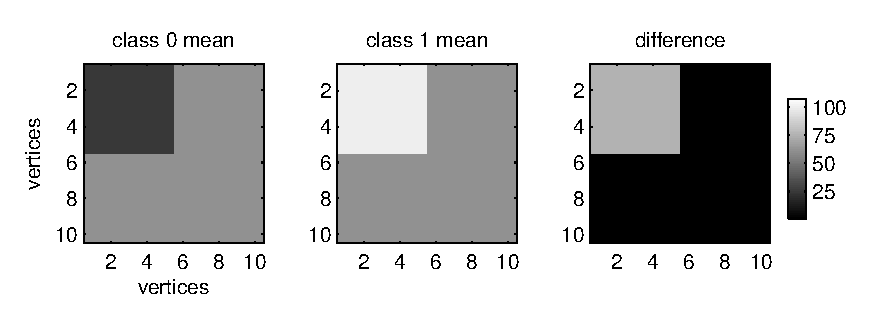
\includegraphics[scale=0.4]{../figs/homo_kidney_egg_model}
\label{fig:homo_subfig1}
}
\subfigure[]{
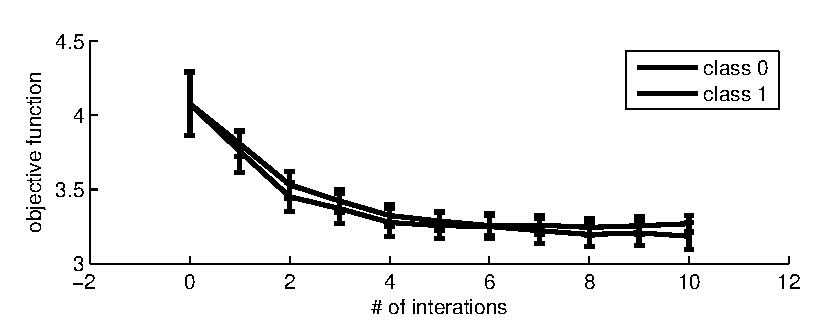
\includegraphics[scale=0.4]{../figs/homo_kidney_egg_obj}
\label{fig:homo_subfig2}
}
\subfigure[Lhat +/- Lstd]{
\includegraphics[scale=1]{../figs/homo_kidney_egg_Lhats}
\label{fig:homo_subfig3}
}
\label{fig:homo}
\caption{Homogeneous-kidney-egg model simulation results. (a) Model: Each edge in the ``kidney'' in both classes has probability $0.5$; in the edge, class 0 edges are sampled with probability $0.25$, and class 1 edges are sampled with probability $0.75$. (b) QAP objective function improves with each iteration of \texttt{QAP}$_1$. (c) But classification performance does not improve.}
\end{figure}



\begin{figure}[ht]
\centering
\subfigure[model]{
\includegraphics[scale=0.4]{../figs/hetero_kidney_egg_model}
\label{fig:hke_subfig1}
}
\subfigure[objective function]{
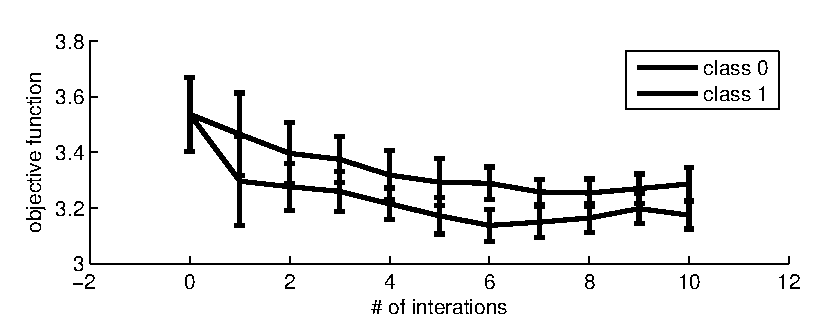
\includegraphics[scale=0.4]{../figs/hetero_kidney_egg_obj}
\label{fig:hke_subfig2}
}
\subfigure[Lhat +/- Lstd]{
\includegraphics[scale=1]{../figs/hetero_kidney_egg_Lhats}
\label{fig:hke_subfig3}
}
\label{fig:hke}
\caption{hetero kidney egg model}
\end{figure}


\begin{figure}[ht]
\centering
\subfigure[model]{
\includegraphics[scale=0.4]{../figs/hetero_model}
\label{fig:hetero_subfig1}
}
\subfigure[objective function]{
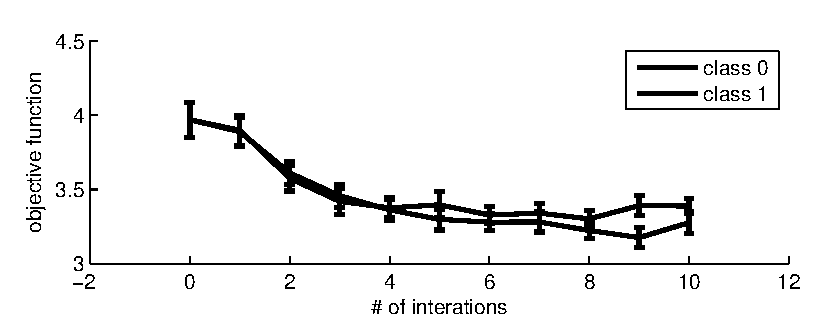
\includegraphics[scale=0.4]{../figs/hetero_obj}
\label{fig:hetero_subfig2}
}
\subfigure[Lhat +/- Lstd]{
\includegraphics[scale=1]{../figs/hetero_Lhats}
\label{fig:hetero_subfig3}
}
\label{fig:hetero}
\caption{hetero model}
\end{figure}


\subsection{LAP vs. QAP} % (fold)
\label{sub:lap_vs_qap}

The LAP approximation for this class problem is given by the following equation:
\begin{align} \label{eq:LAP}
	\mh{Q}_{\text{LAP}} = \argmin_{Q \in \mc{Q}} \norm{A Q\T - B }^2_F,
\end{align}
which is quite similar to QAP, except $A$ is only post-multiplied by $Q$, instead of also being pre-multiplied by $Q$. LAP can be solved exactly as a quadratic problem with linear constraints (as above, one can relax the constraint to the set of doubly stochastic matrices, and still be guaranteed to obtain a permuation matrix). Thus, one can use gradient ascent to to solve a LAP.  The gradient of $f'(Q)=\norm{AQ\T-B}_F^2$ is %:
% \begin{align} \label{eq:grad2}
	$\partial f'/\partial Q = 2A B\T$. 
% \end{align}
Comparing this gradient to that of QAP (Eq. \eqref{eq:grad}), one can see that when $Q^{(k)}$ is the identical matrix, the two gradients are identical.  Thus, if QAP is initialized at the identity matrix, the first iteration is identical to LAP.  This suggests that for certain problems, LAP is both an efficient and useful approximation to graph matching.  We confirm this intuition by substituting QAP with LAP in the above simulations (black line).  As depicted in the above figures, this intuition is consistent with the numerical results. In other words, while naively one might implement an algorithm with exponential time complexity, LAP, which is only quadratic time complexity, will often suffice.


% subsection lap_vs_qap (end)

\subsection{Connectome Classification} % (fold)
\label{sub:connectome_classification}

A ``connectome'' is a graph in which vertices correspond to biological neural units, and edges correspond to connections between the units.  Diffusion Magnetic Resonance (MR) Imaging and related technologies are making the acquisition of MR connectomes routine [cite].  We use 49 subjects from the Baltimore Longitudinal Study on Aging, with acquisition and connectome inference details as reported in [cite].  For each connectome, we obtain a $70 \times 70$ element adjacency matrix, where each element of the matrix encodes the number of streamlines between a pair of regions [FACT cite], ranging between 0 and about 65,000.  Associated with each graph is class label based on the gender of the individual (24 males, 25 females).  Because the vertices are labeled, we can compare the results of having the labels and not having the labels.  As such, we implement the following classification strategies.  In each case, we use a leave-one-out strategy to evaluate performance:

\begin{description}
	\item[\texttt{N/A-QAP}] Using the vertex labels, implement a standard $1$NN classifier, where distance is the norm of the difference between any pair of adjacency matrices.
	\item[\texttt{1-QAP}] Permute only the vertex labels of the test graph, and then implement \texttt{$1$NN$\circ$QAP$_1$}.
	\item[\texttt{48-QAP}] Permuting the vertex labels, then implement \texttt{$1$NN$\circ$QAP$_1$}.
	\item[\texttt{AVG-QAP}] Permuting the vertex labels, \qapa each of the 48 training graphs to the test graph.  Then, given those permuted adjacency matrices, compute the average, and then implement a standard $1$NN classifier.
	\item[\texttt{1NN-GI}] Use the graph invariant approach as described above. We provide the normalized graph invariants as inputs into a number of standard classifiers, including $k$NN, linear classifiers, support vector machines, random forests, and CW. On this data, the CW classifier performed best; we therefore only report its results.
\end{description}

Table \ref{tab:connectome} shows leave-one-out misclassification rates for the various strategies.


\begin{table}[h!]
\caption{MR Connectome Leave-One-Out Misclassification Rates}
\begin{center}
\begin{tabular}{|r|r|r|r|r|}
\hline
\texttt{N/A-QAP} & \texttt{1-QAP} & \texttt{48-QAP} & \texttt{AVG-QAP} & \texttt{1NN-GI}\\
\hline
$20\%$ & $31\%$ & $45\%$ & ?? & $25\%$ \\
    \hline
\end{tabular}
\end{center}
\label{tab:connectome}
\end{table}%


\section{Discussion}


In this work, we have presented a number of approaches one could take to classifier graphs.  Importantly, when the vertex labeling function is unavailable, one must deal with this uncertainty somehow.  We compare a number of approaches on both simulated and connectome data.  A multiple-restart Frank-Wolfe approach to approximating QAP outperforms previous state-of-the-art approaches in terms of approximating the graph matching problem.  Simulations demonstrate that only the first iteration of such an iterative algorithm, starting from the identity matrix, yields classification performance better than chance.  Moreover, the first iteration is identical to LAP, which is a quadratic problem with linear constraints, and therefore can be solved quite easily.  

On a connectome dataset, we compare the performance of various \qap classification algorithms with several graph invariant (GI) based strategies.  Of the algorithms that we tried, a graph invariant approach was most effective, even though, in theory, a QAP based approach could have done better (compare the first and last columns of Table \ref{tab:connectome}).  

These analyses leave many open questions.  Perhaps most interestingly, when might one expect a QAP-based approach to outperform a GI-based approach?  Resorting to a generative model, it should be clear that if the class conditional difference is independent of the vertex labeling function, $\alpha_V$, then there is no reason to even try to implement graph matching.  However, if one believes that the labeling function might convey some class-conditional signal (as in the connectome data), then QAP-based approaches could outperform any approach that ignores the labeling function.  Which QAP-based approach to use in such a scenario, however, will depend on many factors, including the assumed model and computational resources.



% \subsubsection*{Acknowledgments}
% 
% Use unnumbered third level headings for the acknowledgments. All
% acknowledgments go at the end of the paper. Do not include 
% acknowledgments in the anonymized submission, only in the 
% final paper. 


\bibliography{/Users/joshyv/Research/latex/biblist}
\addcontentsline{toc}{section}{References}
%\bibliographystyle{apalike}
\bibliographystyle{ieeetr}
%\bibliographystyle{nature}


% 
% \subsubsection*{References}
% 
% References follow the acknowledgments. Use unnumbered third level heading for
% the references. Any choice of citation style is acceptable as long as you are
% consistent. It is permissible to reduce the font size to `small' (9-point) 
% when listing the references. {\bf Remember that this year you can use
% a ninth page as long as it contains \emph{only} cited references.}
% 
% \small{
% [1] Alexander, J.A. \& Mozer, M.C. (1995) Template-based algorithms
% for connectionist rule extraction. In G. Tesauro, D. S. Touretzky
% and T.K. Leen (eds.), {\it Advances in Neural Information Processing
% Systems 7}, pp. 609-616. Cambridge, MA: MIT Press.
% 
% [2] Bower, J.M. \& Beeman, D. (1995) {\it The Book of GENESIS: Exploring
% Realistic Neural Models with the GEneral NEural SImulation System.}
% New York: TELOS/Springer-Verlag.
% 
% [3] Hasselmo, M.E., Schnell, E. \& Barkai, E. (1995) Dynamics of learning
% and recall at excitatory recurrent synapses and cholinergic modulation
% in rat hippocampal region CA3. {\it Journal of Neuroscience}
% {\bf 15}(7):5249-5262.
% }

\end{document}
